% CREATED BY DAVID FRISK, 2016
\chapter{Sphere Tracing} \label{spheretracing}

	The graphics rendering algorithm the GPU was designed for is called
	Sphere Tracing\cite{Hart1996}. The name comes from the technique where it
	uses spheres to incrementally advance a ray in 3D space. The method of
	advancing rays in general is called Ray Marching which in turn is a subset of
	Ray Tracing\cite{Whitted1980a}. Ray Tracing, then, is a way of wholly or
	partially render the world off of rays, cast from the eye of the observer
	into the scene. Sphere Tracing has been around since at least as early as the
	late eighties\cite{Hart1989} and Ray Tracing as early as the
	sixties\cite{Appel1968}.

	In this chapter the Sphere Tracing algorithm is lifted in detail with
	both definitions and examples. The explanation is based on the the very
	succinct explanation in \cite{Korndorfer2014}. The paper also expands upon
	the original algorithm in some innovative ways. For a more in-depth
	description of the original algorithm see Harts ``\emph{Sphere Tracing: a
	geometric method for the anti-aliased ray tracing of implicit
	surfaces}``\cite{Hart1996}.

	\section{Sphere Tracing} 

		\begin{wrapfigure}{r}{0.48\textwidth}
			\begin{flushright}
				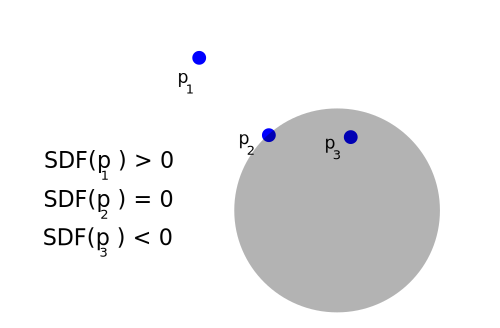
\includegraphics[width=0.9\linewidth]{figure/SDF} 
			\end{flushright}
			\caption{ Signed Distance Function of a sphere, sampled at three points}
			\vspace{40pt}Sphere Tracing
		\end{wrapfigure}

		The Sphere Tracing algorithm uses Signed Distance Functions (SDF).
		$$\text{SDF}:\mathbb{R}^{3}\mapsto\mathbb{R}$$ The ``distance`` is the euclidean distance between a point and the closest point on the implicit surface
		$\text{SDF}^{-1}(0)$. ``signed`` refers to the distance being
		negative when measured on the inside of an object. 

		A common example would be the SDF of a sphere centered at the origin with a
		radius of one. $$\text{SDF}(\vec{v}) = |\vec{v}| - 1$$ We can here see that
		a point $\vec{v}$ exactly on the surface would evaluate to $1 - 1 = 0$
		where any point outside of the sphere is positive and any point inside the
		sphere is negative. In this case the absolute value of the result would also
		describe the smallest distance to the surface but as long as the result is
		the smallest distance \emph{or greater}, the algorithm will work.

		If we define a ray $r$ $$r(s) = \vec{d} \cdot s + \vec{o}$$
		where $\vec{d}$ is the direction of the ray and $\vec{o}$ the origin, then
		$$\text{SDF}\circ r(s) = 0$$ means that the ray intersects a surface at
		exactly distance $s$ from the view point origin. Sampling every SDF in a
		given scene and returning the smallest value yields a function known as a
		distance field.

		\bigskip \noindent Finding the surface can be done by marching point by
		point from the origin along the ray like below: 
		
		$$p_{i+1} = p_i + \vec{d}\cdot \text{SDF}(p_i)$$ 
		
		\vspace{40pt}
		\begin{wrapfigure}{r}{0.48\textwidth}
			\begin{flushright}
				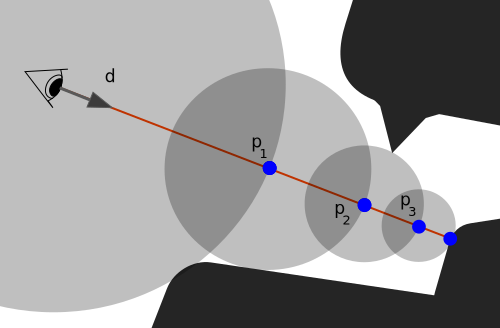
\includegraphics[width=0.9\linewidth]{figure/SDF2} 
			\end{flushright}
			\caption{A single ray marching according to Sphere Tracing}
			\vspace{40pt}
		\end{wrapfigure}

		This is repeated until $\text{SDF}(p_i) \leq \varepsilon$ for a given
		precision limit $\varepsilon$. $\text{SDF}(p_i)$ is the furthest possible
	 distance the ray can march while still not overshooting any potential
		surfaces. The direction to the closest surface point is never known, thus
		$\text{SDF}(p_i)$ can be interpreted as a spherical bound, giving the
		algorithm it's name. The Sphere Trace is performed for each pixel of the
		screen, reversely simulating the light rays entering the lens of an eye or
		camera.

			\subsection{Reflections, refractions and shading}

				Once a point on a surface for a given pixel has been located
				reflections, light, shadows and refractions can be calculated. These sometimes depend on the surface normal which can be approximated with
				the partial derivatives around the surface point given some small delta
				$\delta$. This is the normalized gradient $\vec{g}$ in this point.

				$$\vec{g} = \vec{x}\cdot\frac{\text{SDF}(x+\delta, y, z)}{\delta} +
				\vec{y}\cdot\frac{\text{SDF}(x, y+\delta, z)}{\delta} +
				\vec{z}\cdot\frac{\text{SDF}(x, y, z+\delta)}{\delta} $$

				$$\vec{n} = \frac{\vec{g}}{|\vec{g}|} $$

				A simple way to illuminate the scene could for an example be to use
				Phong Lightning\cite{Phong1975}. But any number of alternative
				algorithms could be used instead to determine the final color. Shadows
				can be determined by doing a new Sphere Trace, towards the sources of
				light to check for obstructions. Same for reflections and refractions
				where further marching in proportionate angles to the angle of
				incidence can determine what objects reflects on the surface.
